%\documentclass[11pt]{article}
%\usepackage{fullpage}
%\usepackage{graphicx}
%\usepackage{adjustbox}
%\usepackage[font=small, labelfont=bf, skip=1pt]{caption}

%\begin{document}

\subsection{External interface requirements}
\subsubsection{User interfaces}
The following mockups represent a basic idea of what the mobile app will look like in the first release. The last one shows instead an idea about the minimal interface of the wearable application. \newline

\begin{figure}[h!]
\centering
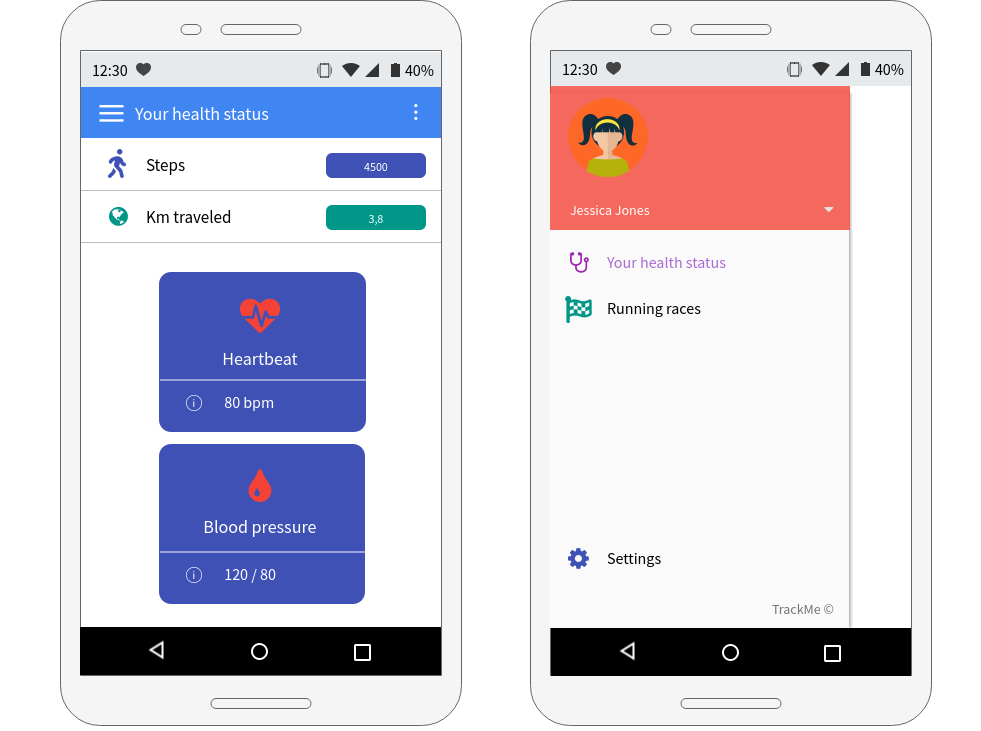
\includegraphics[scale=0.45]{sections/mockups/mockups1,2.png} \newline
\captionof{figure}{[Mockup] - Home page of user's account (the user can monitor his/her own parameters)}	\captionof{figure}{[Mockup] - Side menu \newline}	
\end{figure}

\clearpage

\begin{figure}[h!] \ContinuedFloat
\centering
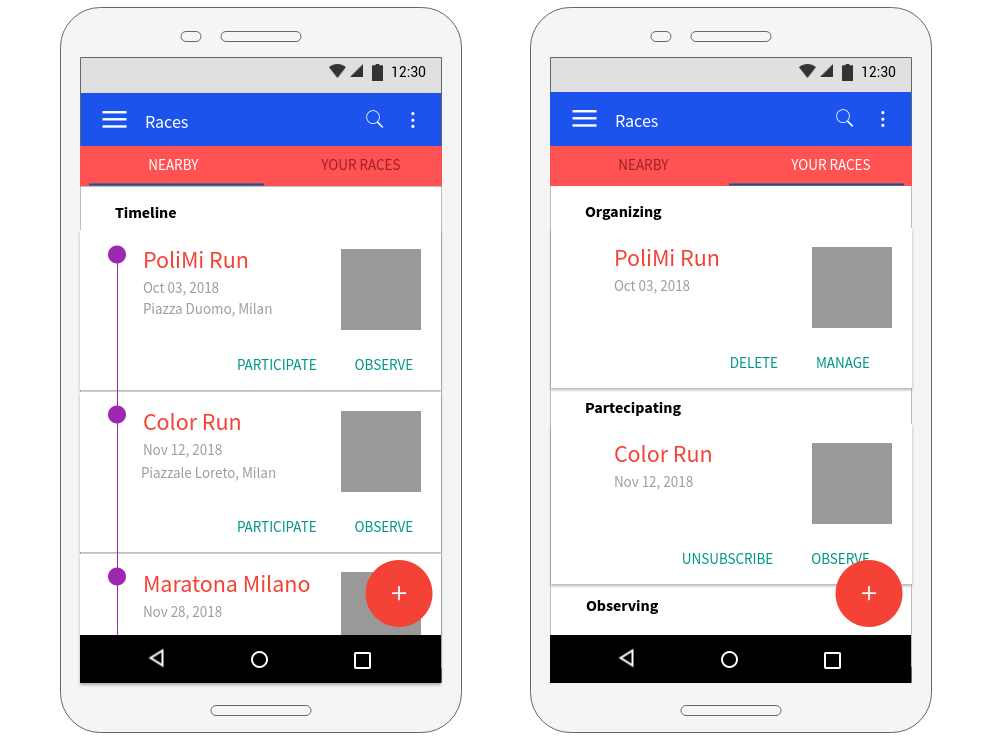
\includegraphics[scale=0.45]{sections/mockups/mockups3,4.png} \newline
\captionof{figure}{[Mockup] - Races screen (NEARBY tab)}
\captionof{figure}{[Mockup] - Races screen (YOUR RACES tab)}
\end{figure}

\begin{figure}[h!] \ContinuedFloat
\centering
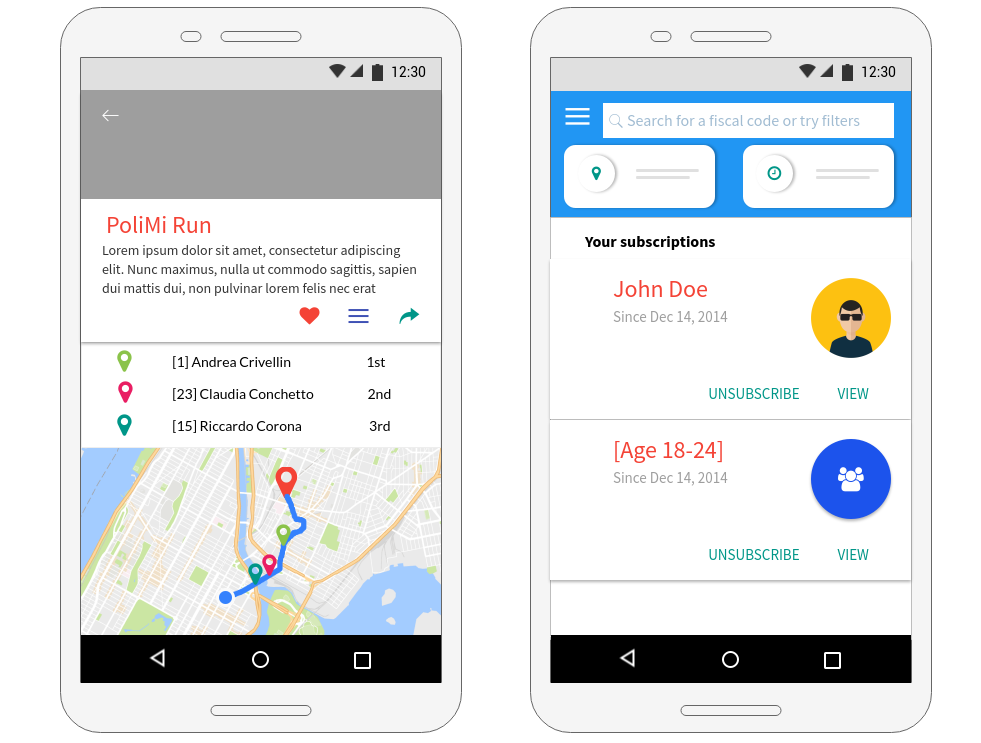
\includegraphics[scale=0.45]{sections/mockups/mockups5,6.png} \newline
\captionof{figure}{[Mockup] - Race overview with leaderboard and track}
\captionof{figure}{[Mockup] - Home page of company's account (the company can search and manage data)}
\end{figure}

\clearpage
	
\begin{figure}[h!] \ContinuedFloat
\centering
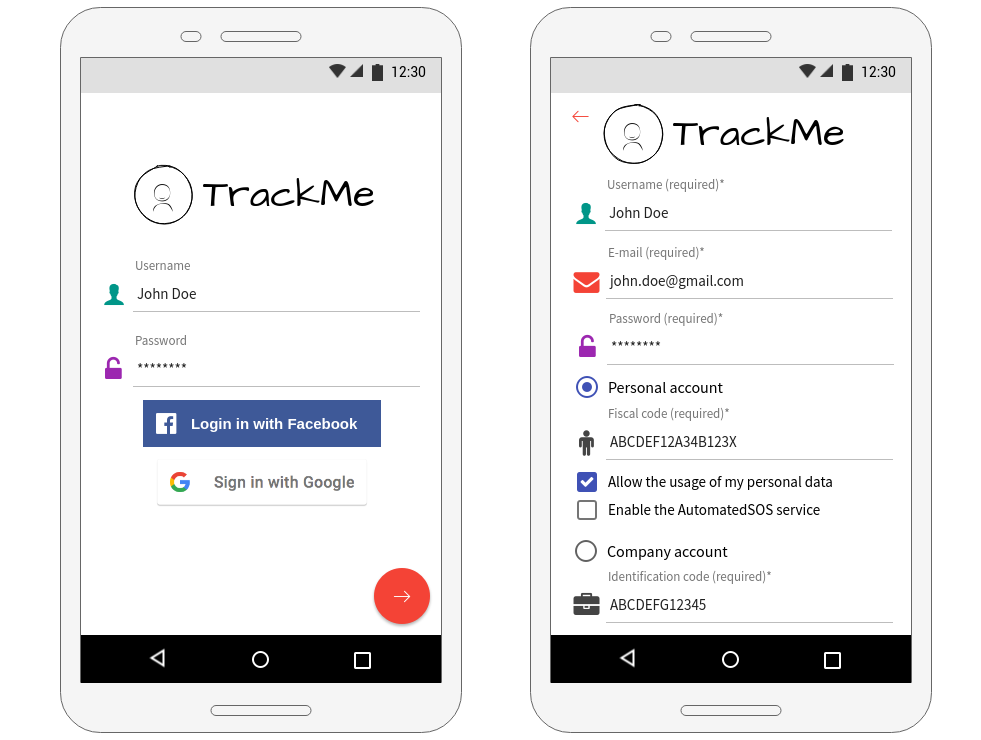
\includegraphics[scale=0.45]{sections/mockups/mockups7,8.png} \newline
\captionof{figure}{[Mockup] - Login screen}
\captionof{figure}{[Mockup] - Registration screen}
\end{figure}
	
\begin{figure}[h!] \ContinuedFloat
\centering
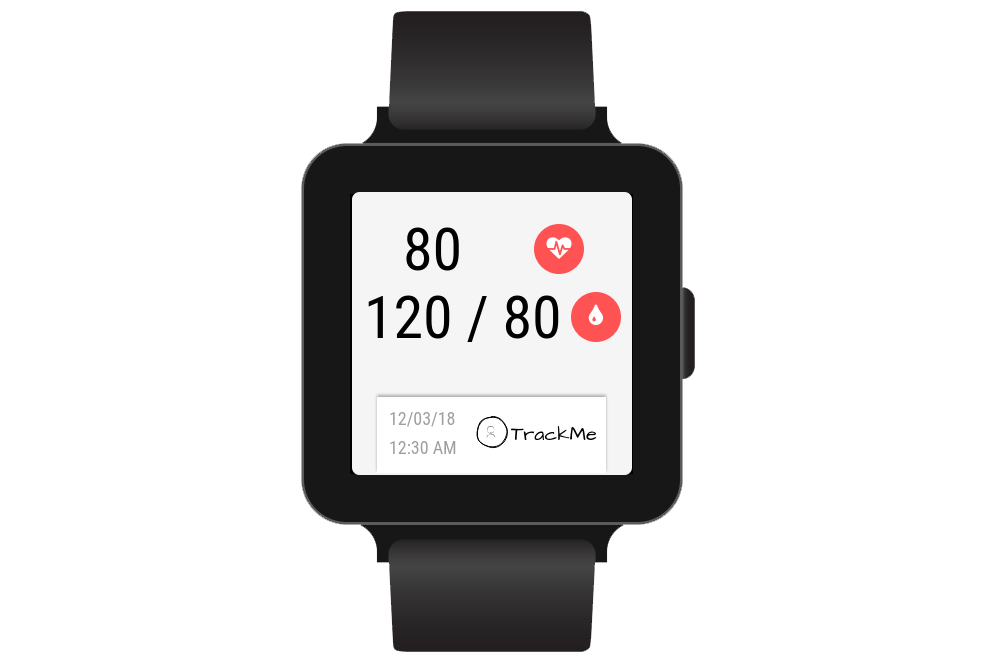
\includegraphics[scale=0.45]{sections/mockups/mockupWatch.png} \newline
\captionof{figure}{[Mockup] - Example of the app screen on a smartwatch}
\end{figure}

\subsubsection{Hardware interfaces}
The application doesn't use any hardware interface, however a smartphone paired with a wearable device like a smartwatch or a fitness tracker is required to use the Data4Help and AutomatedSOS services, and to participate to races using Track4Run (pairing in most cases is made via bluetooth).

The wearable device must have at least the following sensors: GPS, accelerometer, altimeter, gyroscope, heart rate sensor. Other biosensors supported are related to the detection of glucose level, blood pressure, body temperature and ECG and devices equipped with them are highly recommended for a complete experience with TrackMe.

Organizers and spectators of running races, and also third parties can manage their activities without specific hardware requirements (wearable device not required for their tasks).

Users who own a smartwatch with Wear OS or watchOS can also download a TrackMe version specifically designed for this kind of devices.

\subsubsection{Software interfaces}
The application obviously offers a graphical user interface, which allows users to easily communicate with the device.

Furthermore the app uses a city maps external service, suitable for embedding in order to simplify the overall architecture and make it more lightweight. Because the Track4Run service is based on planning, participating and following running races, the app needs accurate real-time informations for mapping the track. Google Maps APIs represent the best choice in order to provide an effective service. Google Maps also provides the users with the reliable location information they need throughout the world.

\subsubsection{Communication interface}
The app uses the following communication interfaces:
\begin{itemize}
\item Internet connection for communication of data.
\item RESTful APIs and JSON data format for communication over HTTP.
\item SDK Maps for Android, SDK Maps for iOS and API Maps JavaScript in order to allow an efficient Google Maps integration (these APIs allow to add an interactive and personalizable map in a mobile application, on Android and iOS).
\item Interface with the push service(s) via own APIs in order to allow the app to send and receive push notifications to users' devices (both iOS and Android are supported).
\item Interface with SMS and voice gateway provider via standard APIs in order to allow the app to send SMS and to make phone calls (useful for the AutomatedSOS service).
\item Wearable APIs in order to get data from smartphones, fitness trackers and other wearable devices.
\end{itemize}

\subsection{Scenarios}
\subsubsection{Scenario 1}
Aurora is a non-profit organization that deals with disabled young people. Aurora's board of directors decided to use TrackMe to support medicians in their work and monitor the health status of patients in a more efficient way. Most of the patients, according with their parents, decided to download the app on their smartphone. Aurora's medicians were able to estimate the average course of the heartbeat, blood pressure, body temperature, glucose level and ECG of patients just searching for anonymous data using the age filter (18-21 years old) and the location filter (via Aurora 2, Perugia) and subscribing to the search results.

\subsubsection{Scenario 2}
Davide is the athletic trainer for the under 21 athletes of Milano Atletica. He decided to organize a competition between his student, so he launched TrackMe and created a new running race in the "Your running races" section, using the "+" button. He selected the location of the sport center (via Cimabue, Milan) and established the date of the race (15/11/2018) and the closing date of the registrations (14/11/2018). He obviously decided to select the participants sending them invites to join the competition.

Giovanni, one of his students, immediately joined the competition but unluckily he was not able to compete due to an injury. Through the "MANAGE" option Davide was able to mark him as "disqualified" in order to effectively know the participants in the race and monitor their performances.

\subsubsection{Scenario 3}
Lidia is an elderly woman who loves walking. His grandson Matteo suggested her to download the TrackMe app on her smartphone paired with her fitness tracker, in order to monitor her own activities and health status and also to make sure his grandmother receives assistance in case of health problems.

One day, during a walk, Lidia felt sick and collapsed on the ground. TrackMe detected an abnormality in the heartbeat and called immediately the 112, sending also an SMS with her position, heart rate and blood pressure. The ambulance intervened a few minutes later and Lidia was successfully rescued.

\subsection{Functional Requirements}
\textbf{[G1] - Users and third parties can be recognized by providing a form with their data} \newline

[R1] -  The usernames used in the system are unique to every user and third party. \newline

[D1] - Third parties own an alphanumerical code received from a TrackMe administrator used to verify their identities and match them with the company account. \newline

[R2] - Users and third parties can create an account by compiling a form. \newline

\hspace{\parindent}[R2.1] - The form should contain the following: username, password, choice between personal and third party account, other anagraphical info (for the user) or company info (for the third party). \newline

[R3] - Third parties must provide an identification alphanumerical code to confirm their identity. \newline

[R4] - Users and third parties can log in to the application by providing the combination of a username and a password that match an account. \newline

\hspace{-\parindent}\textbf{[G2] - Allow third parties to access to the data of some specific individuals} \newline

[D2] - Device sensors can provide accurate data to the app. \newline

[R5] - Third parties can search for specified data by filling the search bar with the fiscal code of a specific user. \newline

[R6] - A notify is sent to the selected user, who can accept or refuse the sharing of data with the specific company. \newline

[R7] - A message is sent to the third party, containing user's data if he/she allowed the sharing or a notification of refuse otherwise. \newline

[R8] - Users under 18 years old can't be shown in the results of a search. \newline

\hspace{-\parindent}\textbf{[G3] - Allow third parties to access to anonymized data of groups of individuals} \newline

[R9] - Third parties can search for anonymized data of a specific group of users by selecting search filters (location, age, sex, time slot). \newline

[R10] - Anonymized data are shown just if the research produces at least 1000 results. \newline

\hspace{-\parindent}\textbf{[G4] - Allow third parties to subscribe to new data and to receive them as soon as they are produced} \newline

[R11] - Third parties can flag an option to subscribe to new data of a specific user when they receive his/her data (the user already allowed the data sharing), or they can subscribe to get results of a research with specific filters as soon as they are produced. \newline

[R12] - Third parties can manage their subscriptions and set the frequency with which obtaining data for a specific subscription by selecting it and editing preferences. \newline

\hspace{-\parindent}\textbf{[G5] - Allow the users, through the AutomatedSOS service, to come help by an ambulance when such parameters fall below certain thresholds} \newline

[D3] - TrackMe is affiliated with NUE 112 (Numero Unico per le Emergenze) to offer assistance in Europe, and with 911 to offer assistance in the USA. \newline

[R13] - Users can manage the subscription to the AutomatedSOS service through a specific option in the settings menu. \newline

[R14] - Old users (60+ years old) are automatically subscribed to the AutomatedSOS service since their registration. \newline

[R15] - The app calls autonomously the NUE (or 911) when such parameters fall below certain thresholds, and sends concurrently user's data (GPS location and health status parameters) via SMS. \newline

\hspace{-\parindent}\textbf{[G6] - Allow racing organizers, through the Track4Run service, to manage runs and define a path for runs} \newline

[R16] - Users can create races by defining name, date, time, start point, stages and arrival point, and selecting the method of participation (open or by invitation) and the date and time of expiration for registrations. They can also add other organizers as collaboratos: selected users will receive a notify and they will see the race in their management section. \newline

\hspace{\parindent}[R16.1] - If a race by invitation is selected, a private link to a registration page is generated. \newline

\hspace{\parindent}[R16.2] - The organizer can specify a maximum of 10 stages. \newline

\hspace{\parindent}[R16.3] - The distance between start and arrival points (stages included) cannot exceeds 50kms, otherwise a warning popup is shown and the organizer is invited to change at least one of them before continuing. \newline

[R17] - Organizers can choose one of the routes calculated by the system. \newline

[R18] - The system allows the organizers to sign an enrolled runner as "present" and to disqualify a runner by signing him/her as "disqualified". \newline

[R19] - Users can manage their organizing races in a management section in the app. \newline

\hspace{\parindent}[R18.1] - Organizers can postpone or delete a run. A notification is sent to participants and spectators. \newline

\hspace{-\parindent}\textbf{[G7] - Allow racing participants to enroll runs} \newline

[R20] - Users can visualize nearby races or search for a specific run by searching for the name or location of the race. \newline

[D4] - The run can be joined only by persons enrolled through the app. \newline

[D5] - If it is required a payment to enroll a run, an external service will guarantee secure transactions and receipts by e-mail. \newline

[R21] - Runners can join a race through the race overview by clicking the "Participate" button. For races by invitation the button is visible just to invited users following the registration link. \newline

\hspace{\parindent}[R20.1] - If it's specified that some payment is required, it will be committed to an external service. \newline

[R22] - When the race starts, the participant have to wear his/her wearable device with Data4Help installed. \newline

\hspace{-\parindent}\textbf{[G8] - Allow racing spectators to see on a map the position of all runners during the run} \newline

[R23] - Users can become spectators of a race through the race overview by clicking the "Observe" button. \newline

[R24] - For the duration of the race is always possible to see in the event page the map with markers, associated to runners' name through numbers, and a live leaderboard showing names, order numbers and possible disqualifications. \newline

[R25] - A marker is on the track iff it corresponds to a user enrolled, signed as "present" at the run with his/her wearable device with Data4Help installed and not disqualified. \newline

[R26] - The track represented is the one chosen by the organizer of the run. \newline

[R27] - Markers move according to the corresponding persons' movement, as reported by the location service. \newline

\hspace{-\parindent}\textbf{[G9] - Allow users to monitor their own health status} \newline

[R28] - Users can visualize their own health status in the home page section of the app. \newline
\newpage

\subsubsection{Use case diagrams}
\begin{figure}[h!]
\centering
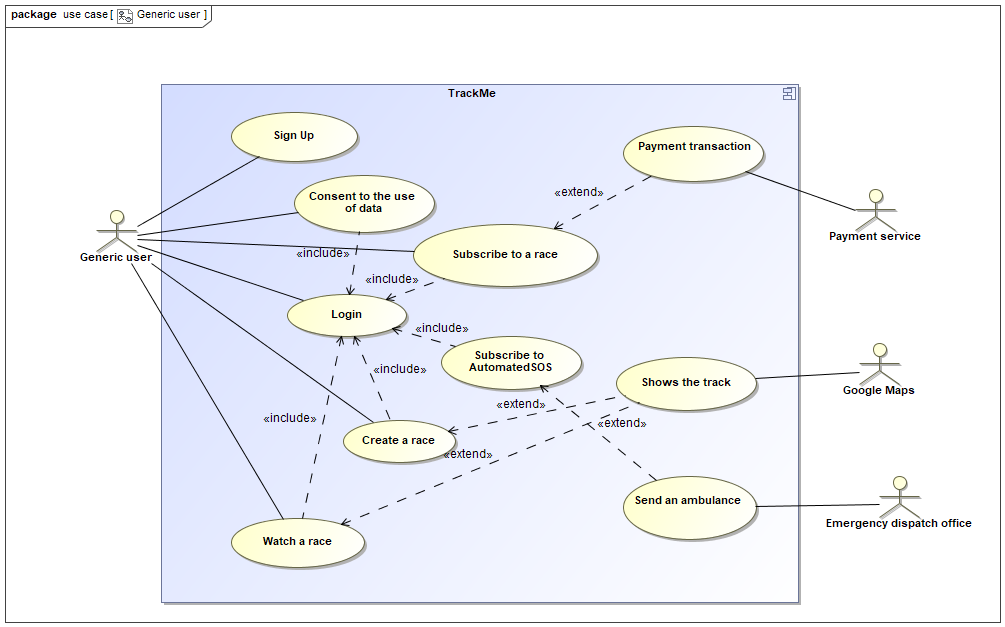
\includegraphics[scale=0.44]{sections/diagrams/Generic_user.png} \newline
\captionof{figure}{Use case diagram from user's point of view}
\end{figure}

\begin{figure}[h!] \ContinuedFloat
\centering
\includegraphics[scale=0.44]{sections/diagrams/Third_Party.png} \newline
\captionof{figure}{Use case diagram from third party's point of view}
\end{figure}

\clearpage

\begin{table}[]
\begin{adjustbox}{width=\textwidth}
\footnotesize
\begin{tabular}{|p{0.17\textwidth}|p{0.83\textwidth}|}
\hline
\textbf{Name}             &  Sign Up\\ \hline
\textbf{Actor}            &  User, third party\\ \hline
\textbf{Entry conditions} &  The user/third party has installed the application on the device\\ \hline
\textbf{Events flow}      &
	\begin{itemize}
		\item[1.] Click on the "CREATE AN ACCOUNT" button
		\item[2.] Fill all the mandatory fields and provide the necessary information
		\item[3.] Click on the "CONFIRM" button
		\item[4.] The system sends an e-mail of confirmation to the specified e-mail address and saves the data
	\end{itemize}\\ \hline
\textbf{Exit conditions}  &  The user/third party has successfully registered and now he/she’s able to use the application\\ \hline
\textbf{Exceptions}       &
	\begin{itemize}
		\item[1.] The user/third party already signed up
		\item[2.] The user/third party didn’t fill all of the mandatory fields with valid data
		\item[3.] The username is already taken
		\item[4.] The e-mail is already registered
	\end{itemize}
	All the exceptions are handled by notifying the user/third party and taking him/her back to the sign up activity\\ \hline
\end{tabular}
\end{adjustbox}
\end{table}

\begin{table}[]
\begin{adjustbox}{width=\textwidth}
\footnotesize
\begin{tabular}{|p{0.17\textwidth}|p{0.83\textwidth}|}
\hline
\textbf{Name}             &  Login\\ \hline
\textbf{Actor}            &  User, third party\\ \hline
\textbf{Entry conditions} &  The user/third party is previously successfully signed up and has the application installed on the device\\ \hline
\textbf{Events flow}      &
	\begin{itemize}
		\item[1.] Enter credentials in the “Username” and “Password” fields of the home page or choose one between the Google and Facebook autentication buttons
		\item[2.] Click on the "LOGIN" button [if the choice was to log in manually]
		\item[3.] The user/third party is successfully logged in his/her profile and the system automatically redirects him/her to the related home page
	\end{itemize}\\ \hline
\textbf{Exit conditions}  &  The user/third party is successfully redirected to the home page\\ \hline
\textbf{Exceptions}       &
	\begin{itemize}
		\item[1.] The user/third party enters invalid username
		\item[2.] The user/third party enters invalid password
	\end{itemize}
	All the exceptions are handled by notifying the user/third party and taking him/her back to the login 	activity\\ \hline
\end{tabular}
\end{adjustbox}
\end{table}

\begin{table}[]
\begin{adjustbox}{width=\textwidth}
\footnotesize
\begin{tabular}{|p{0.17\textwidth}|p{0.83\textwidth}|}
\hline
\textbf{Name}             &  Consent to the use of data\\ \hline
\textbf{Actor}            &  User\\ \hline
\textbf{Entry conditions} &  The user receives a push notification telling him that a specific third party wants to access to his data\\ \hline
\textbf{Events flow}      &
	\begin{itemize}
		\item[1.] Click on the push notification
		\item[2.] Click on the "I AGREE" button
		\item[3.] The user successfully allowed the usage of his data and the system redirects him to his home page
	\end{itemize}\\ \hline
\textbf{Exit conditions}  &  The user is successfully redirected to the home page\\ \hline
\textbf{Exceptions}       &
	\begin{itemize}
		\item[1.] The user swipe away the notification
	\end{itemize}
	The exception is handled showing to the user the choice screen at the opening of the app\\ \hline
\end{tabular}
\end{adjustbox}
\end{table}

\begin{table}[]
\begin{adjustbox}{width=\textwidth}
\footnotesize
\begin{tabular}{|p{0.17\textwidth}|p{0.83\textwidth}|}
\hline
\textbf{Name}             &  Watch a race\\ \hline
\textbf{Actor}            &  User\\ \hline
\textbf{Entry conditions} &  The user has already logged in\\ \hline
\textbf{Events flow}      &
	\begin{itemize}
		\item[1.] Swipe right to show the side menu
		\item[2.] Click on the "Running races" voice
		\item[3.] Search for a specific run using the search button on the upper bar or explore nearby races
		\item[4.] Click on the "OBSERVE" button
		\item[5.] The user successfully chose the race to watch and the system saves the race in user's "Observing" section and shows the user the specific running race page
	\end{itemize}\\ \hline
\textbf{Exit conditions}  &  The system saves the race in user's "Observing" section and shows the user the specific running race page\\ \hline
\textbf{Exceptions}       &
	\begin{itemize}
		\item[1.] The user can't find the race he is searching for
	\end{itemize}\\ \hline
\end{tabular}
\end{adjustbox}
\end{table}

\begin{table}[]
\begin{adjustbox}{width=\textwidth}
\footnotesize
\begin{tabular}{|p{0.17\textwidth}|p{0.83\textwidth}|}
\hline
\textbf{Name}             &  Create a race\\ \hline
\textbf{Actor}            &  User\\ \hline
\textbf{Entry conditions} &  The user has already logged in\\ \hline
\textbf{Events flow}      &
	\begin{itemize}
		\item[1.] Swipe right to show the side menu
		\item[2.] Click on the "Running races" voice
		\item[3.] Click on the "+" button
		\item[4.] Fill all the mandatory fields (name of the competition, date, time, start point, arrival point, date and time of expiration for registrations)
		\item[5.] Choose one of the purposed routes
		\item[6.] Choose between open or by invitation race selecting the corresponding radio button
		\item[7.] Click on the "CONFIRM" button
		\item[8.] Select people to invite choosing them from the list which appears [if the choice was the by invitation race]
		\item[9.] Click on the "CONTINUE" button [if the choice was the by invitation race]
		\item[10.] The user successfully created the race and the system saves the race in user's "Organizing" section and shows the user the specific running race page
	\end{itemize}\\ \hline
\textbf{Exit conditions}  &  The system saves the race in user's "Organizing" section and shows the user the specific running race page\\ \hline
\textbf{Exceptions}       &
	\begin{itemize}
		\item[1.] The user didn’t fill all of the mandatory fields with valid data
		\item[2.] The distance between start and arrival point exceeds 50kms
	\end{itemize}
	All the exceptions are handled by notifying the user and inviting him to modify data\\ \hline
\end{tabular}
\end{adjustbox}
\end{table}

\begin{table}[]
\begin{adjustbox}{width=\textwidth}
\footnotesize
\begin{tabular}{|p{0.17\textwidth}|p{0.83\textwidth}|}
\hline
\textbf{Name}             &  Manage a race\\ \hline
\textbf{Actor}            &  User\\ \hline
\textbf{Entry conditions} &  The user has already logged in and he wants to modify a running race previously created\\ \hline
\textbf{Events flow}      &
	\begin{itemize}
		\item[1.] Swipe right to show the side menu
		\item[2.] Click on the "Running races" voice
		\item[3.] Switch to the "YOUR RACES" tab
		\item[4.] If the choice is to delete a race click on the "DELETE" button, otherwise click on the "MANAGE" button
		\item[5.] Modify the information which need to be changed editing the relative field: start point, stages, arrival point, date, time, date and time of expiration for registrations, or choose a participant and click on the "DISQUALIFY" button to mark him as "disqualified" [if the chose was to manage]
		\item[6.] Click on the "CONFIRM" button [if the chose was to manage]
		\item[7.] The user successfully deleted/modified the race and the system shows the user the specific running race page
	\end{itemize}\\ \hline
\textbf{Exit conditions}  &  The system shows the user the specific running race page or the "YOUR RACES" tab if the choice was to delete the race\\ \hline
\textbf{Exceptions}       &
	\begin{itemize}
		\item[1.] The user didn’t fill all of the mandatory fields with valid data
		\item[2.] The distance between start and arrival point exceeds 50kms
	\end{itemize}
	All the exceptions are handled by notifying the user and inviting him to modify data\\ \hline
\end{tabular}
\end{adjustbox}
\end{table}

\begin{table}[]
\begin{adjustbox}{width=\textwidth}
\footnotesize
\begin{tabular}{|p{0.17\textwidth}|p{0.83\textwidth}|}
\hline
\textbf{Name}             &  Subscribe to a race\\ \hline
\textbf{Actor}            &  User\\ \hline
\textbf{Entry conditions} &  The user has already logged in\\ \hline
\textbf{Events flow}      &
	\begin{itemize}
		\item[1.] Swipe right to show the side menu
		\item[2.] Click on the "Running races" voice
		\item[3.] Search for a specific run using the search button on the upper bar or explore nearby races
		\item[4.] Click on the "PARTICIPATE" button
		\item[5.] If a payment is required it's necessary to provide it
		\item[6.] The user successfully chose the race to join and the system saves the race in user's "Participating" section and shows the user the specific running race page
	\end{itemize}\\ \hline
\textbf{Exit conditions}  &  The system saves the race in user's "Participating" section and shows the user the specific running race page\\ \hline
\textbf{Exceptions}       &
	\begin{itemize}
		\item[1.] The user can't find the race he is searching for
	\end{itemize}\\ \hline
\end{tabular}
\end{adjustbox}
\end{table}

\begin{table}[]
\begin{adjustbox}{width=\textwidth}
\footnotesize
\begin{tabular}{|p{0.17\textwidth}|p{0.83\textwidth}|}
\hline
\textbf{Name}             &  Subscribe to AutomatedSOS\\ \hline
\textbf{Actor}            &  User\\ \hline
\textbf{Entry conditions} &  The user has already logged in\\ \hline
\textbf{Events flow}      &
	\begin{itemize}
		\item[1.] Swipe right to show the side menu
		\item[2.] Click on the "Settings" voice
		\item[3.] Scroll the page searching for the checkbox related to the AutomatedSOS subscription
		\item[4.] Select the checkbox
		\item[5.] Click on the "SAVE" button to save preferences
		\item[6.] The user successfully subscribed to AutomatedSOS and the system automatically redirects him to the home page
	\end{itemize}\\ \hline
\textbf{Exit conditions}  &  The user is successfully redirected to the home page\\ \hline
\textbf{Exceptions}       &  /\\ \hline
\end{tabular}
\end{adjustbox}
\end{table}

\begin{table}[]
\begin{adjustbox}{width=\textwidth}
\footnotesize
\begin{tabular}{|p{0.17\textwidth}|p{0.83\textwidth}|}
\hline
\textbf{Name}             &  Choose a path\\ \hline
\textbf{Actor}            &  User\\ \hline
\textbf{Entry conditions} &  The user is organizing a running race and he has already set correctly start and arrival point\\ \hline
\textbf{Events flow}      &
	\begin{itemize}
		\item[1.] The user chooses one of the listed tracks
		\item[2.] The system saves the data
	\end{itemize}\\ \hline
\textbf{Exit conditions}  &  The chosen path is saved as track for the race\\ \hline
\textbf{Exceptions}       &  /\\ \hline
\end{tabular}
\end{adjustbox}
\end{table}

\begin{table}[]
\begin{adjustbox}{width=\textwidth}
\footnotesize
\begin{tabular}{|p{0.17\textwidth}|p{0.83\textwidth}|}
\hline
\textbf{Name}             &  Payment transaction\\ \hline
\textbf{Actor}            &  User\\ \hline
\textbf{Entry conditions} &  The user has already logged in and wants to participate to a running race which requires a payment subscription\\ \hline
\textbf{Events flow}      &
	\begin{itemize}
		\item[1.] The user chooses what kind of payment he wants to make
		\item[2.] The user provides the system with all the required information for making a 	payment
	\end{itemize}\\ \hline
\textbf{Exit conditions}  &  The payment is successful\\ \hline
\textbf{Exceptions}       &
	\begin{itemize}
		\item[1.] The user did not enter a valid data
	\end{itemize}\\ \hline
\end{tabular}
\end{adjustbox}
\end{table}

\begin{table}[]
\begin{adjustbox}{width=\textwidth}
\footnotesize
\begin{tabular}{|p{0.17\textwidth}|p{0.83\textwidth}|}
\hline
\textbf{Name}             &  Send an ambulance\\ \hline
\textbf{Actor}            &  TrackMe\\ \hline
\textbf{Entry conditions} &  Some of the health status parameters of the user fall below specific thresholds (hearth rate, blood pressure, body temperature)\\ \hline
\textbf{Events flow}      &
	\begin{itemize}
		\item[1.] The app transcript data about location and health status as a textual message
		\item[2.] Using the GPS coordinates, the app recognizes the phone number to contact (112 or 911)
		\item[3.] The app calls the phone number and concurrently sends user's data via SMS
	\end{itemize}\\ \hline
\textbf{Exit conditions}  &  Someone answers the call\\ \hline
\textbf{Exceptions}       &  /\\ \hline
\end{tabular}
\end{adjustbox}
\end{table}

\begin{table}[]
\begin{adjustbox}{width=\textwidth}
\footnotesize
\begin{tabular}{|p{0.17\textwidth}|p{0.83\textwidth}|}
\hline
\textbf{Name}             &  Calculate the path\\ \hline
\textbf{Actor}            &  TrackMe\\ \hline
\textbf{Entry conditions} &  The user wants to participate to a running race and has already selected start point and arrival point (and optionally intermediate stages)\\ \hline
\textbf{Events flow}      &
	\begin{itemize}
		\item[1.] The app gathers all the information provided by external map services
		\item[2.] The app calculates routes according with user's specifications
		\item[3.] The system saves the data
	\end{itemize}\\ \hline
\textbf{Exit conditions}  &  The calculated routes are presented to the user\\ \hline
\textbf{Exceptions}       &  /\\ \hline
\end{tabular}
\end{adjustbox}
\end{table}

\begin{table}[]
\begin{adjustbox}{width=\textwidth}
\footnotesize
\begin{tabular}{|p{0.17\textwidth}|p{0.83\textwidth}|}
\hline
\textbf{Name}             &  Show the path\\ \hline
\textbf{Actor}            &  TrackMe\\ \hline
\textbf{Entry conditions} &  The user clicks on a running race\\ \hline
\textbf{Events flow}      &
	\begin{itemize}
		\item[1.] The app gathers all the information provided by external map services
		\item[2.] Comparing date and time of the event with actual date and time, the app shows:
		\begin{itemize}
		\item An empty leaderboard and an empty track if the actual date and time precede those of the expiration for registrations
		\item The leaderboard with participants' info and their markers at the start point of the track if the actual date and time preced those of the race
		\item The leaderboard with participants' info and their markers at the arrival point of the track if the actual date and time follow those of the end of the race
		\item If the race is in progress, the app gathers all the information about participants' position provided by their devices and shows their markers moving on the track, upgrading the leaderboard
		\end{itemize}
	\end{itemize}\\ \hline
\textbf{Exit conditions}  &  The race screen is correctly shown\\ \hline
\textbf{Exceptions}       &
	\begin{itemize}
		\item[1.] One or more users' devices are broken and can't provide an accurate GPS position
	\end{itemize}
	The exception is managed leaving user's marker in the position of the last correct measurement and considering him as stopped (organizators will manually adjust the leaderboard in the end)\\ \hline
\end{tabular}
\end{adjustbox}
\end{table}

\begin{table}[]
\begin{adjustbox}{width=\textwidth}
\footnotesize
\begin{tabular}{|p{0.17\textwidth}|p{0.83\textwidth}|}
\hline
\textbf{Name}             &  Subscribe to specific individuals data\\ \hline
\textbf{Actor}            &  Third party\\ \hline
\textbf{Entry conditions} &  The third party has already logged in\\ \hline
\textbf{Events flow}      &
	\begin{itemize}
		\item[1.] Search for a fiscal code using the search bar in the home page
		\item[2.] Click on the username associated with the searched fiscal code
		\item[3.] Click on the "OK" button in the confirmation message which is displayed
		\item[4.] The system sends a push notification to the selected user, who can accept or refuse the sharing of his data
		\item[5.] Click on the push notification received from the user to view his fist data if he had consented, or the rejection message otherwise
		\item[6.] Choose the radio button corresponding to the frequency with which obtaining data from the user (once every hour, day, week or month) [if the user allowed the data sharing]
		\item[7.] Click on the "SAVE" button [if the user allowed the data sharing]
		\item[8.] The system saves a link to the users' data in third party's "Your subscriptions" section of the home page [if the user allowed the data sharing] and redirects the third party to the home page
	\end{itemize}\\ \hline
\textbf{Exit conditions}  &  The system saves a link to the users' data in third party's "Your subscriptions" section and redirects the third party to the home page successfully\\ \hline
\textbf{Exceptions}       &
	\begin{itemize}
		\item[1.] The fiscal code doesn't exist in the data base
		\item[2.] The user refuses the data sharing
	\end{itemize}\\ \hline
\end{tabular}
\end{adjustbox}
\end{table}

\begin{table}[]
\begin{adjustbox}{width=\textwidth}
\footnotesize
\begin{tabular}{|p{0.17\textwidth}|p{0.83\textwidth}|}
\hline
\textbf{Name}             &  Subscribe to anonymized groups data\\ \hline
\textbf{Actor}            &  Third party\\ \hline
\textbf{Entry conditions} &  The third party has already logged in\\ \hline
\textbf{Events flow}      &
	\begin{itemize}
		\item[1.] Select one of the suggested search filters in the home page by clicking it
		\item[2.] Set the filter specifying the data (e.g. "Milan" for the location filter)
		\item[3.] [Optional] Repeat the previous steps choosing other filters
		\item[4.] Scroll the page and select one of the displayed results
		\item[5.] Choose the radio button corresponding to the frequency with which obtaining data from the group (once every hour, day, week or month) in the confirmation message which is displayed
		\item[6.] Click on the "SUBSCRIBE" button in the confirmation message
		\item[7.] The system saves a link to the group's data in third party's "Your subscriptions" section of the home page and redirects the third party to the home page
	\end{itemize}\\ \hline
\textbf{Exit conditions}  &  The system saves a link to the group's data in third party's "Your subscriptions" section and redirects the third party to the home page successfully\\ \hline
\textbf{Exceptions}       &
	\begin{itemize}
		\item[1.] No groups are shown (there are less then 1000 results and a group can't be created)
	\end{itemize}\\ \hline
\end{tabular}
\end{adjustbox}
\end{table}

\begin{table}[]
\begin{adjustbox}{width=\textwidth}
\footnotesize
\begin{tabular}{|p{0.17\textwidth}|p{0.83\textwidth}|}
\hline
\textbf{Name}             &  Send data request\\ \hline
\textbf{Actor}            &  TrackMe\\ \hline
\textbf{Entry conditions} &  A third party has already selected a user from which to obtain data\\ \hline
\textbf{Events flow}      &
	\begin{itemize}
		\item[1.] The app retrieves the user's profile from the data base
		\item[2.] The app creates an association table with the request and the user's profile
		\item[3.] The app sends to the user a push notification
		\item[4.] Once the user clicks the button corresponding to his decision to share or not his data, the app retrieves the third party's profile from the request using the association table
		\item[5.] The system sends to the third party a push notification with user's data or with a message of refuse
	\end{itemize}\\ \hline
\textbf{Exit conditions}  &  The third party receives successfully the push notification\\ \hline
\textbf{Exceptions}       &  /\\ \hline
\end{tabular}
\end{adjustbox}
\end{table}

\begin{table}[]
\begin{adjustbox}{width=\textwidth}
\footnotesize
\begin{tabular}{|p{0.17\textwidth}|p{0.83\textwidth}|}
\hline
\textbf{Name}             &  Log in\\ \hline
\textbf{Actor}            &  Administrator\\ \hline
\textbf{Entry conditions} &  /\\ \hline
\textbf{Events flow}      &
	\begin{itemize}
		\item[1.] The administrator enters his/her credentials in the “Username” and “Password” fields of the home page
		\item[2.] The administrator clicks on the "LOGIN" button
		\item[3.] The administrator is successfully logged in his/her profile and the system automatically redirects him/her to the related home page
	\end{itemize}\\ \hline
\textbf{Exit conditions}  &  The administrator is successfully redirected to the options menu\\ \hline
\textbf{Exceptions}       &
	\begin{itemize}
		\item[1.] The administrator enters invalid username
		\item[2.] The administrator enters invalid password
	\end{itemize}
	All the exceptions are handled by notifying the administrator and taking him/her back to the login 	activity\\ \hline
\end{tabular}
\end{adjustbox}
\end{table}

\begin{table}[]
\begin{adjustbox}{width=\textwidth}
\footnotesize
\begin{tabular}{|p{0.17\textwidth}|p{0.83\textwidth}|}
\hline
\textbf{Name}             &  Change forms\\ \hline
\textbf{Actor}            &  Administrator\\ \hline
\textbf{Entry conditions} &  The administrator has already logged in\\ \hline
\textbf{Events flow}      &
	\begin{itemize}
		\item[1.] The administrator opens the option menu
		\item[2.] The administrator chooses the option "Change forms"
		\item[3.] The administrator selects one form to modify
		\item[4.] The administrator can add/remove/modify fields and buttons
		\item[5.] The administrator clicks on the "SAVE" button
		\item[6.] The administrator clicks on the "PROCEED" button in the confirmation message which is displayed
		\item[7.] The system saves the data
	\end{itemize}\\ \hline
\textbf{Exit conditions}  &  The selected form is modified\\ \hline
\textbf{Exceptions}       &  /\\ \hline
\end{tabular}
\end{adjustbox}
\end{table}

\clearpage

\subsection{Performance requirements}
The system is provided to serve fairly great number of users simultaneously. Because of the nature of the application, especially for what concerns the AutomatedSOS service, we have to guarantee quick, reactive and correct responses. When health status parameters fall below certain thresholds the app guarantees a reaction time of less then 5 seconds to contact the NUE (or 911).

\subsection{Design constraints}
\subsubsection{Standards compliance}
\begin{itemize}
\item The app requests only the absolute minimum permissions that it needs to support core functionalities.
\item The mobile app supports both landscape and portrait orientations (if possible). Orientations expose largely the same features and actions and preserve functional parity. Minor changes in content
or views are acceptable. The smartwatch app fits to the dimension of the device.
\end{itemize}

\subsubsection{Hardware limitations}
As previously mentioned in the "Hardware interfaces" section, the app requires a device with a GPS sensor and a wearable device with at least the following sensors: GPS, accelerometer, altimeter, gyroscope, heart rate sensor (biosensor related to the detection of glucose level, blood pressure, body temperature and ECG also supported and recommended). Both iOS and Android are supported, and the connection required can be based on the following technologies: 2G, 3G, 4G, LTE.

\subsubsection{Other constraints}
Regulatory policies are respected: the app share user's data just with third parties allowed by the user himself, and he can also manage his concessions. Data are not used for commercial purpose.

User's payment informations could be asked in particular situations (organization of some special running races) but the app will use them only for fees and rides payments and will not share them with anyone (neither third parties allowed to receive user's data).

\subsection{Software system attributes}
\subsubsection{Reliability}
The application must be available 24/7. Because of the nature of the app, especially for what concerns the AutomatedSOS service, deviations are not tolerated and system's maintenances must be communicated to users (both personal and third parties accounts) via mail at least 1 day before.

\subsubsection{Availability}
In order to guarantee high degree of availability, system of redundant servers may be considered. In this way, if possibly one server fails, the other one will be ready to take over. The system is expected to be
available 99.99\% of the time.

\subsubsection{Security}
Users' credentials and payments informations should be confidentially stored and encrypted. Security of the data and of the communications between users and app is a primary concern.

\subsubsection{Maintainability}
In order to guarantee a good maintainability of the app, the code will be simplified as much as possible, and always commented both with natural language (english) and a first order logic based language (when possible). Design patterns will be used and all the documentation will be provided. Furthermore, the app will always been tested before a new release and changelogs will be generated for each new version of the system.

\subsubsection{Compatibility}
\begin{itemize}
\item Android versions supported: 5.0 (Lollipop) and following.
\item iOS versions supported: iOS 7 and following.
\item WearOS (related to Android watches) and watchOS (related to Apple watches) supported in all versions.
\end{itemize}

%\end{document}